\documentclass{article}
\usepackage{graphicx} % Required for inserting images
\usepackage{amsfonts}
\usepackage{amsmath, amssymb}
\allowdisplaybreaks
\begin{document}
\begin{center} \huge Finding Change in Launch Angle \\
\end{center}
Motivation: When trying to change the launch angle of the cannon, one method is clicking and dragging the cannon up or down. Assuming the cannon is successfully clicked, the following argument lets us find how far up or down the angle of elevation of the cannon should be altered.\vspace{\baselineskip}\\
Consider the following diagram: \vspace{\baselineskip}\\
\begin{figure}[h]
	\centering	
	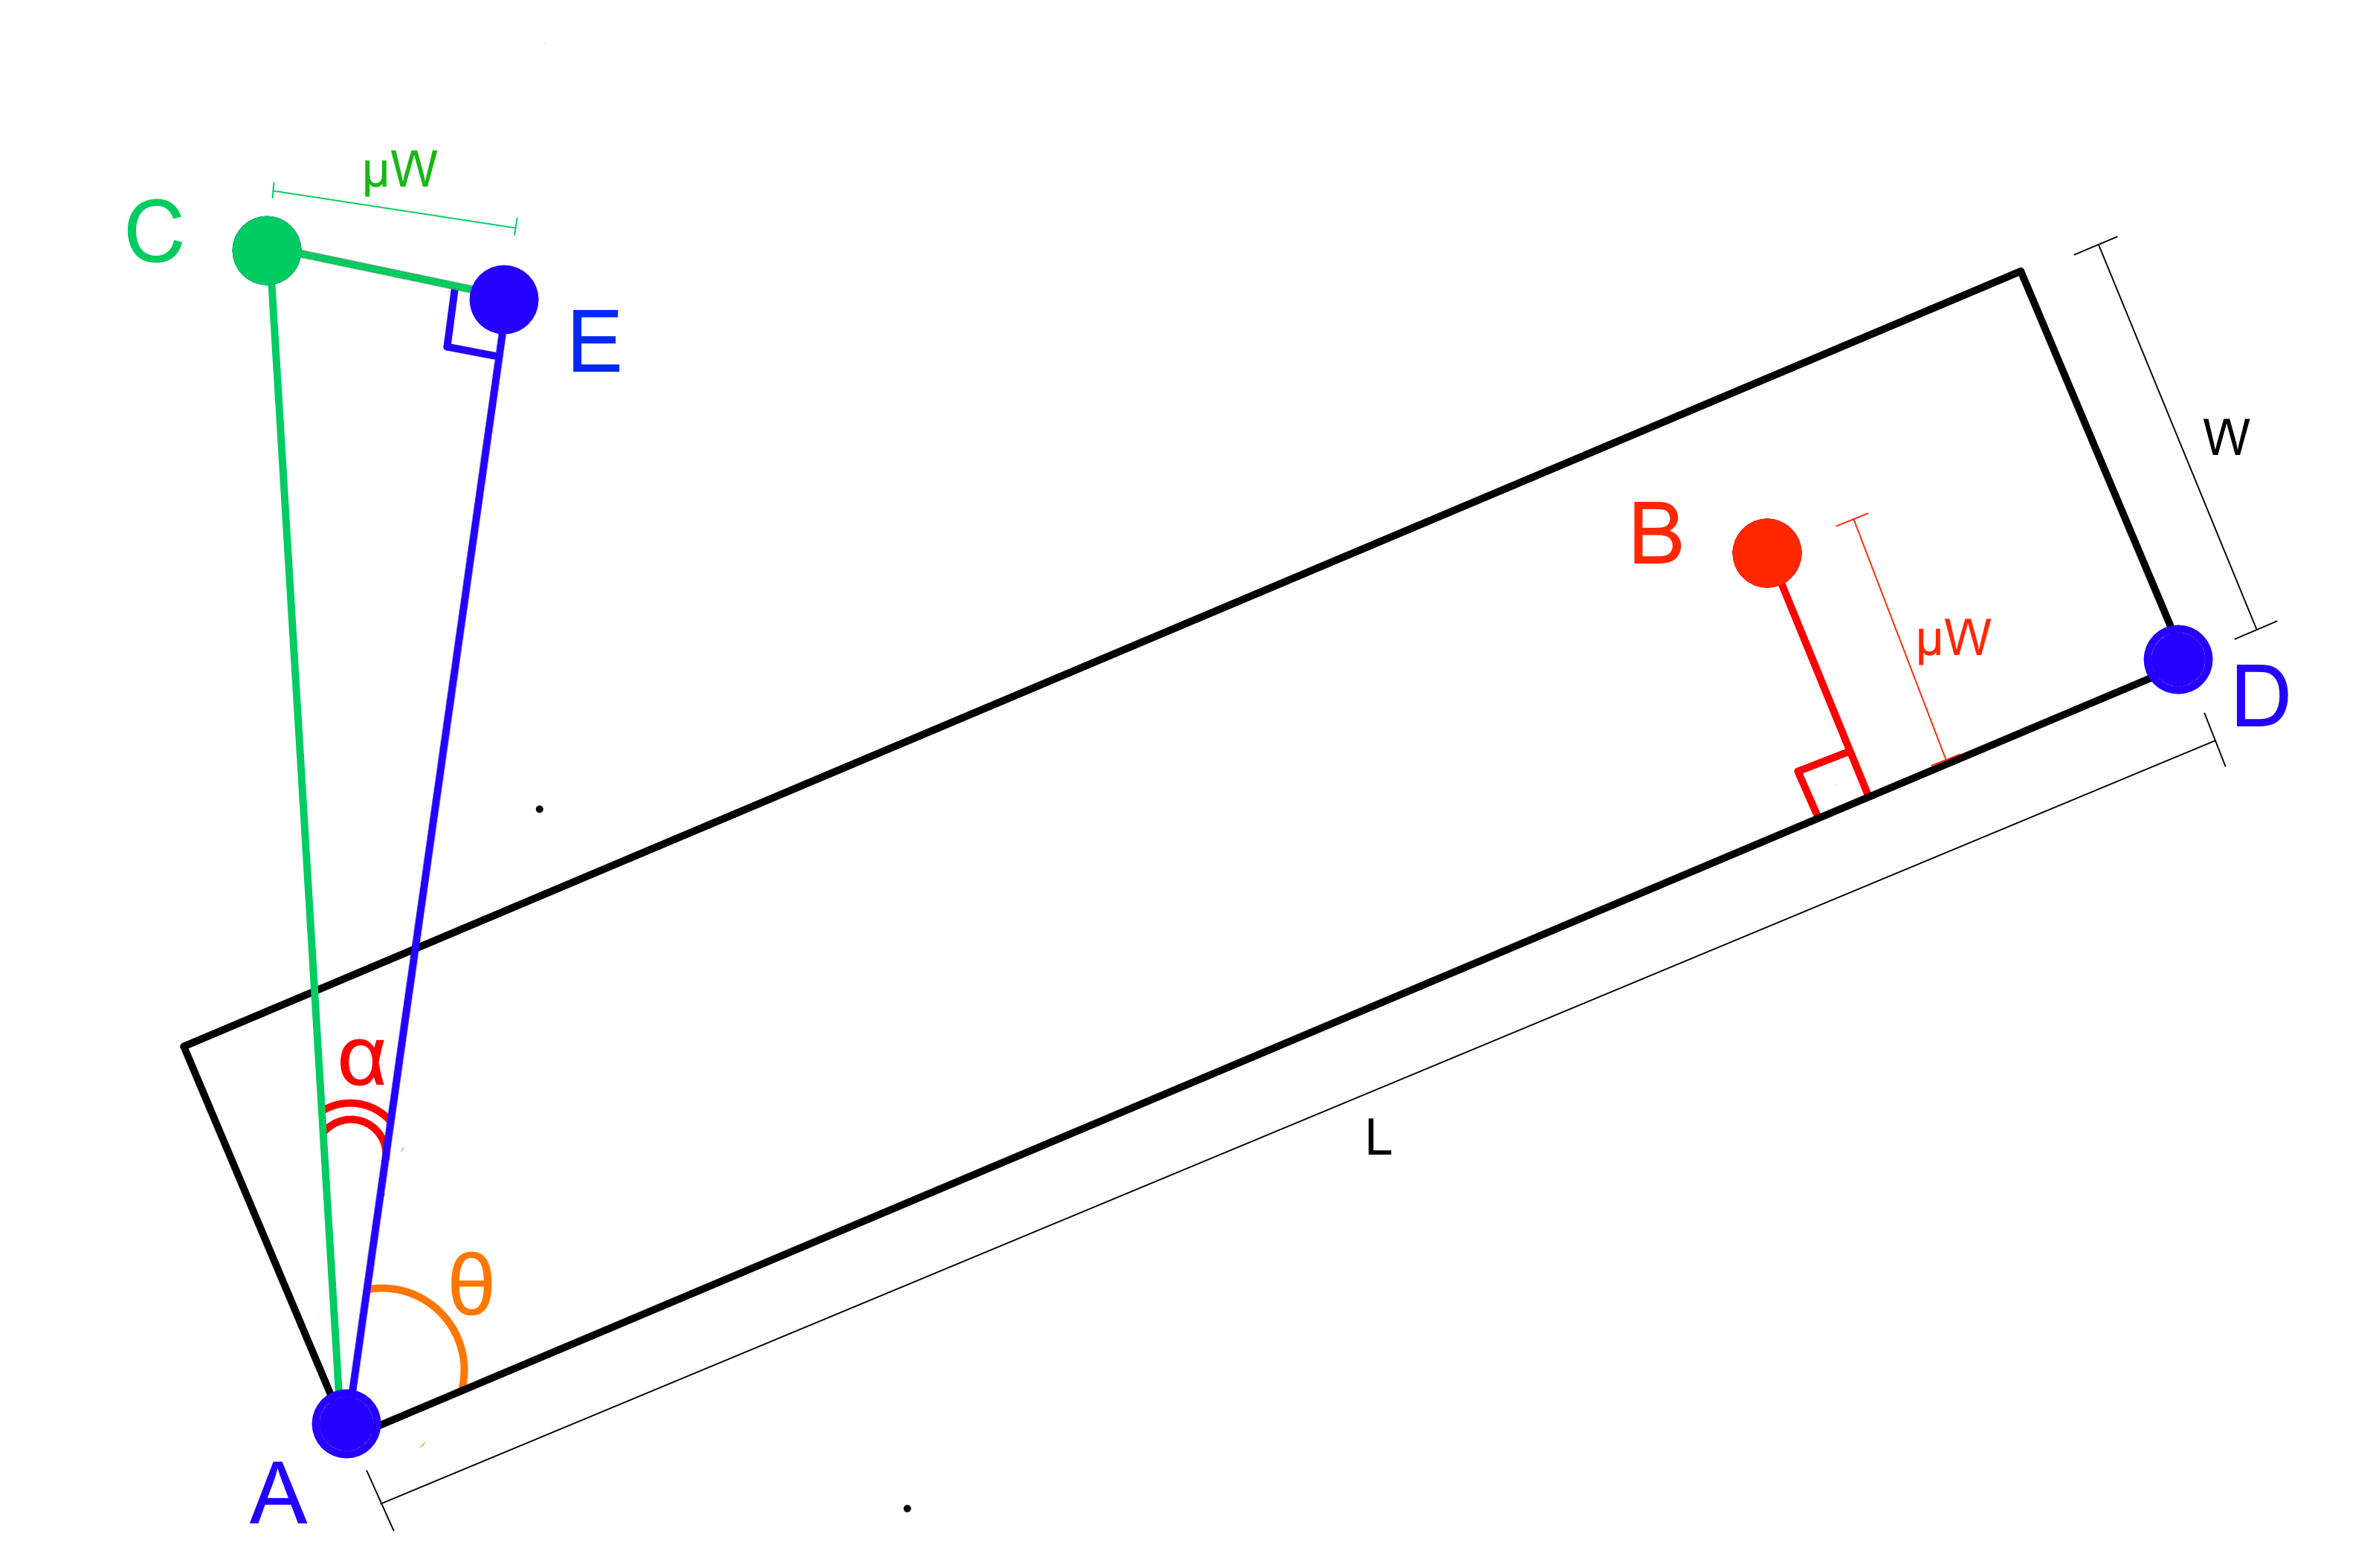
\includegraphics[scale=0.08]{Images/DragFunction1.png}
	\caption{Overview of the whole cannon}
\end{figure} \vspace{\baselineskip}\\
Point $B$ represents where the user would have clicked the cannon, and point $C$ represents where the user would have dragged the mouse to. The general thought process is to find point $E$ such that the $CE$ has a length of $\mu W$, equal to the segment that passes through $B$ and is perpendicular to $AD$. The angle between $AE$ and $AD$, $\theta$, is the change in angle of elevation. \vspace{\baselineskip}\\
Note that the value of $\mu$ would have been previously evaluated when deciding \emph{whether} the user had clicked the cannon or not.\vspace{\baselineskip}\\
Let $$\overrightarrow{OA} = 
\begin{pmatrix}
	a_1\\
	a_2\\
\end{pmatrix}, \
\overrightarrow{OB} = 
\begin{pmatrix}
	b_1\\
	b_2\\
\end{pmatrix}, \
\overrightarrow{OC} = 
\begin{pmatrix}
	c_1\\
	c_2\\
\end{pmatrix}, \
\overrightarrow{OD} = 
\begin{pmatrix}
	d_1\\
	d_2\\
\end{pmatrix}\text{ and }
\overrightarrow{OE} = 
\begin{pmatrix}
	e_1\\
	e_2\\
\end{pmatrix}$$
where $O$ represents the origin point of our coordinate system. Also note that $a_1, \ a_2, \ b_1, \ b_2, \ c_1, \ c_2, \ d_1 \ \text{ and } d_2$ are known.\vspace{\baselineskip}\\
Therefore, $$\overrightarrow{AC} = 
\begin{pmatrix}
	c_1 - a_1\\
	c_2 - a_2
\end{pmatrix}$$
Let $\alpha = \angle CAE$ such that $\alpha \in [0, \frac{\pi}{2}]$ as per Figure 1. Therefore, $\sin{\alpha} = \frac{|\overrightarrow{CE}|}{|\overrightarrow{AC}|} = \frac{\mu W}{|\overrightarrow{AC}|}$ where $|\overrightarrow{AC}| = \sqrt{(c_1 - a_1)^2 + (c_2 - a_2)^2}.$ Therefore we can conclude that $\alpha = \arcsin{\left(\frac{\mu W}{|\overrightarrow{AC}|}\right)}$. \vspace{\baselineskip}\\
Using Figure 1 again we can see that $|\overrightarrow{AE}| = |\overrightarrow{AC}|\cos{\alpha}.$\vspace{\baselineskip}\\
Now consider the following diagram: \vspace{\baselineskip}\\
\begin{figure}[h]
	\centering	
	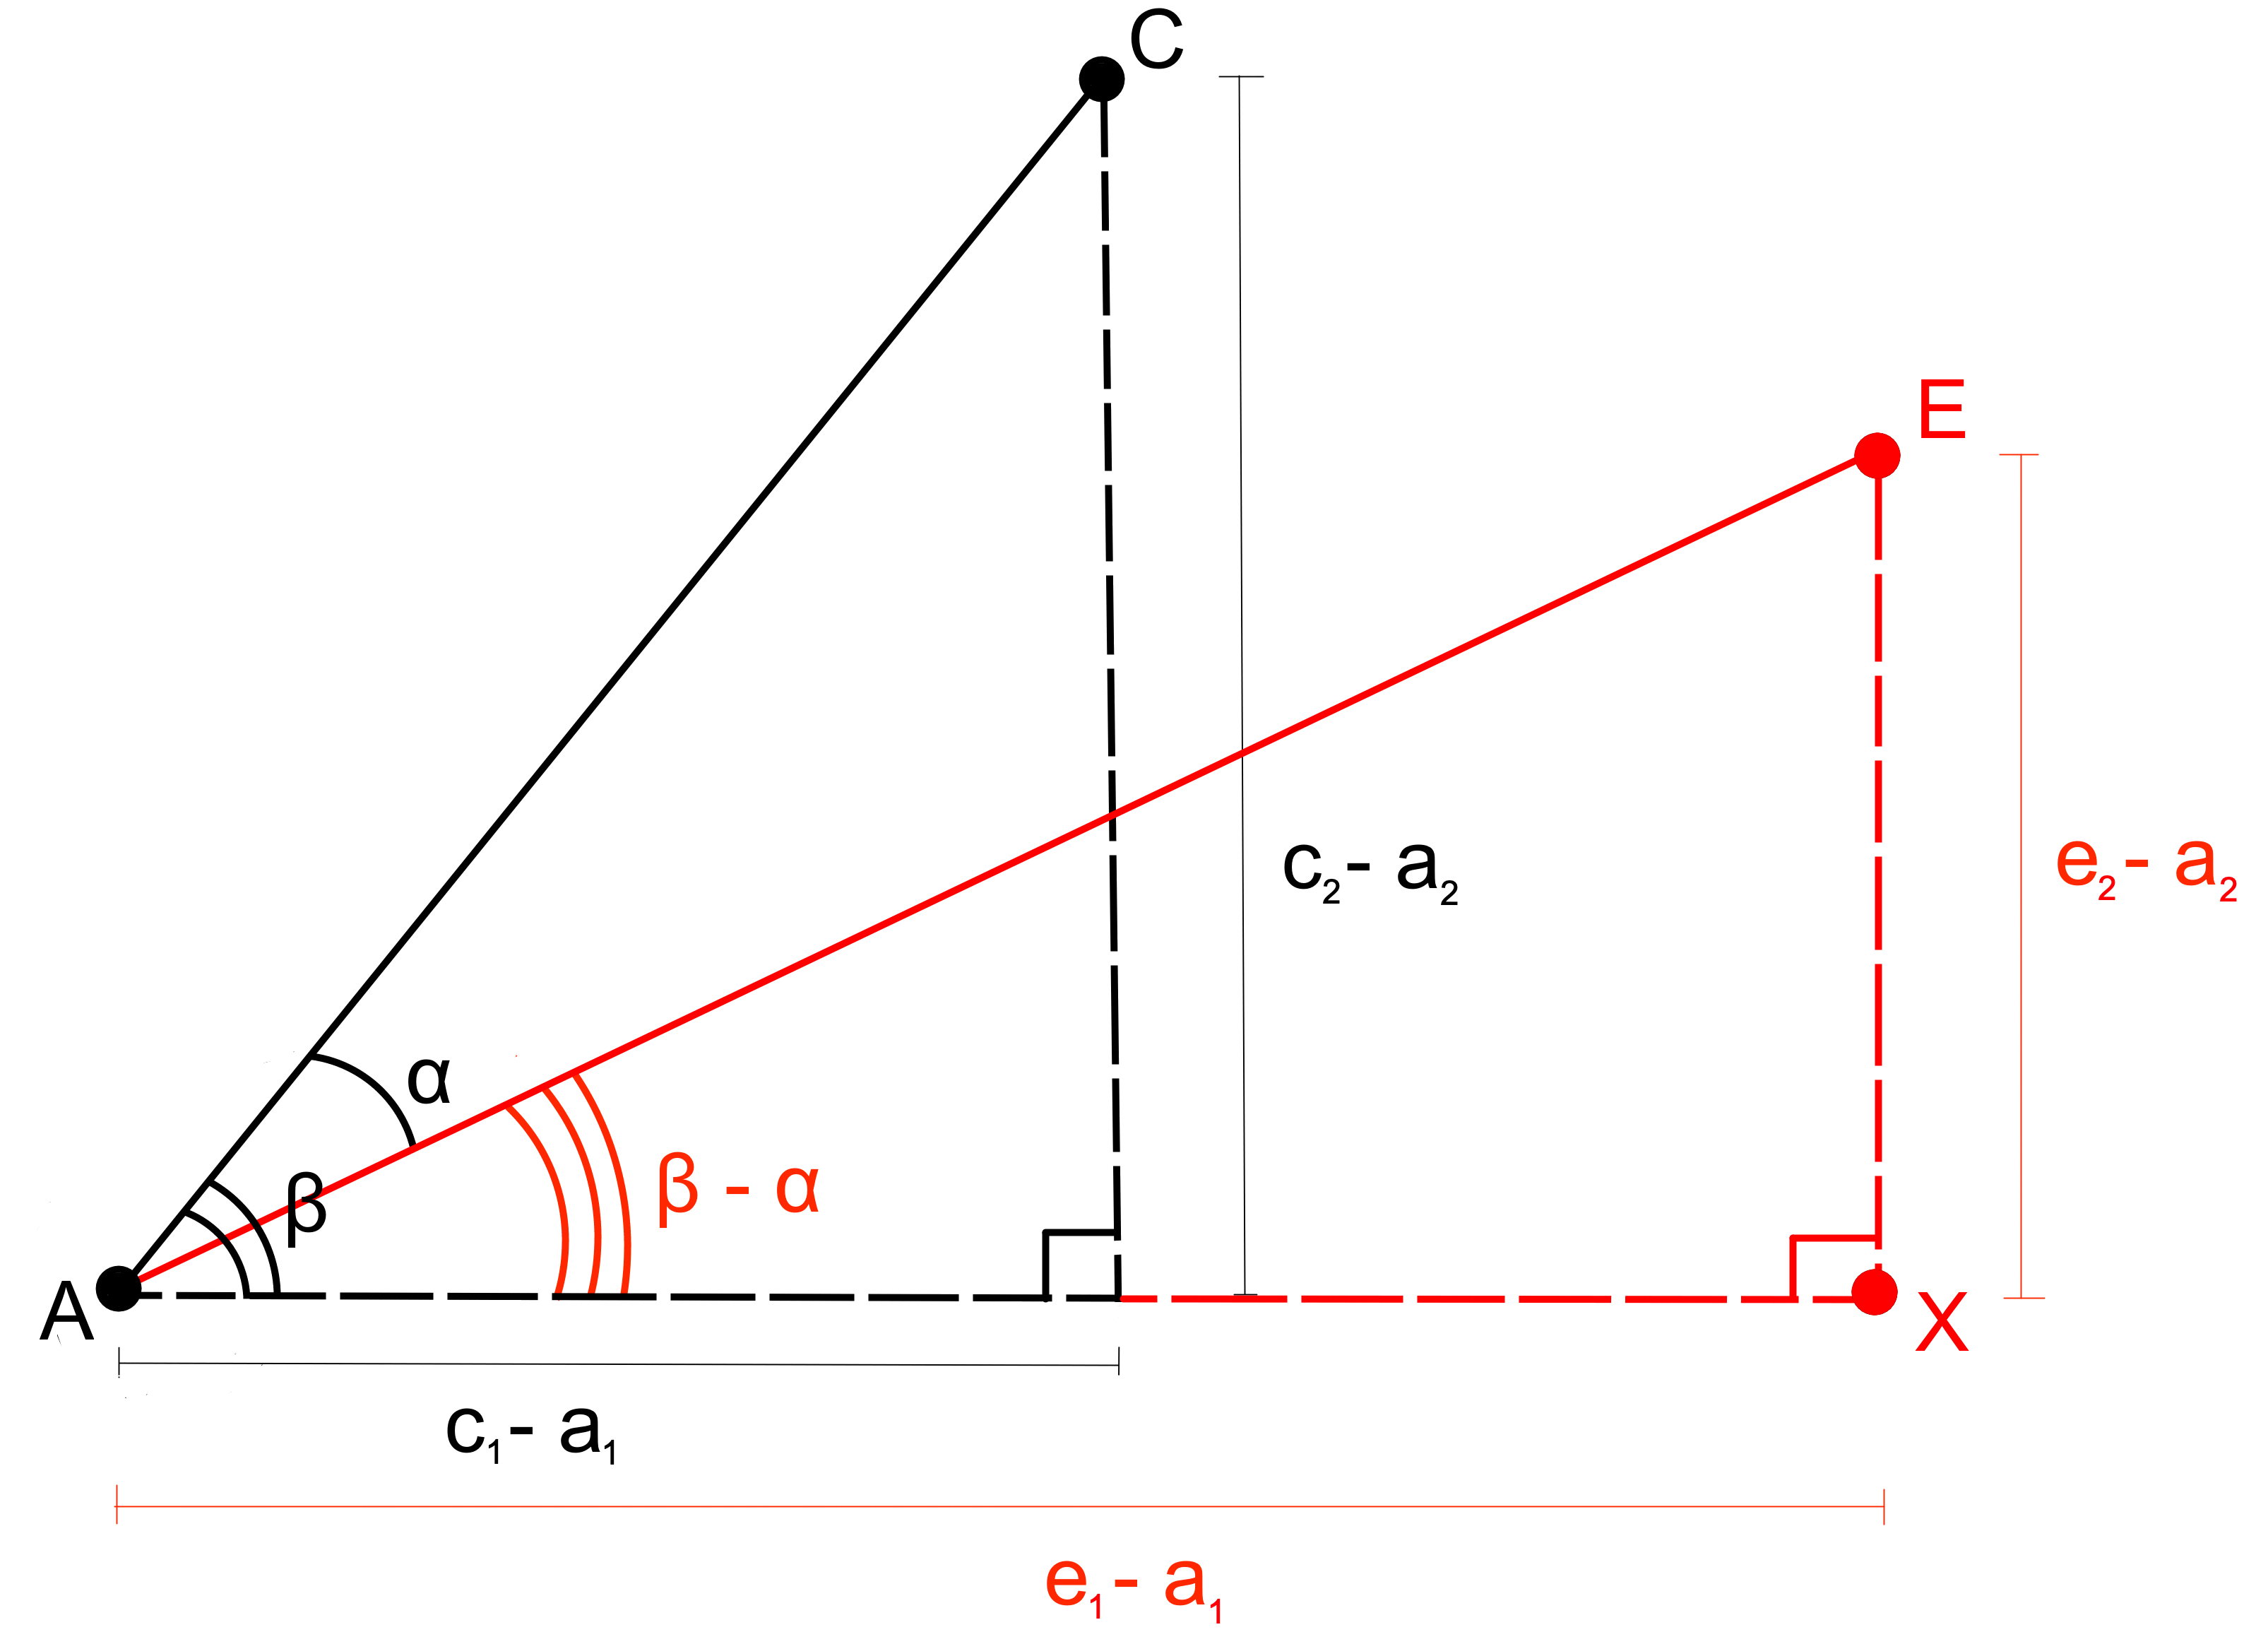
\includegraphics[scale=0.08]{Images/DragFunction2.png}
	\caption{Focusing on line segments \emph{AC} and \emph{AE}}
\end{figure} \vspace{\baselineskip}\\
Recall that $\alpha$ has already been defined as $\angle CAE$. We can also define $\beta$ to be $\angle CAX$ and therefore infer that $\angle EAX = \beta - \alpha$ as indicated in Figure 2.\vspace{\baselineskip}\\
We can say that $\beta = \arctan{\left(\frac{c_2 - a_2}{c_1 - a_1}\right)}$ by inspecting Figure 2. \vspace{\baselineskip}\\
We can finally see that	
\begin{align*}
\cos{(\beta - \alpha)} &= \frac{e_1 - a_1}{|\overrightarrow{AE}|}\\
\implies e_1 &= |\overrightarrow{AE}| \cos{(\beta - \alpha)} + a_1.
\end{align*}

Similarly $$e_2 = |\overrightarrow{AE}| \sin{(\beta - \alpha)} + a_2.$$
\vspace{\baselineskip}\\
So we can say that $\overrightarrow{OE} = 
\begin{pmatrix}
	|\overrightarrow{AE}| \cos{(\beta - \alpha)} + a_1 \\
	|\overrightarrow{AE}| \sin{(\beta - \alpha)} + a_2
\end{pmatrix}$\vspace{\baselineskip}\\
Consider the dot product between $\overrightarrow{AC}$ and $\overrightarrow{AE}.$\vspace{\baselineskip}\\
\begin{align*}
\overrightarrow{AC} \cdot \overrightarrow{AE} &= |\overrightarrow{AE}||\overrightarrow{AC}| \cos{\theta}\\
\implies \cos{\theta} &= \frac{\overrightarrow{AC} \cdot \overrightarrow{AE}}{|\overrightarrow{AE}||\overrightarrow{AC}|}\\
\implies \theta &= \arccos{\left( \frac{\overrightarrow{AC} \cdot \overrightarrow{AE}}{|\overrightarrow{AE}||\overrightarrow{AC}|}\right)}.
\end{align*}

\end{document}